\documentclass[13pt,a4paper]{article}
\usepackage{a4wide,amssymb,epsfig,latexsym,multicol,array,hhline,fancyhdr}
\usepackage{amsmath}
\usepackage{amsfonts}
\usepackage{lastpage}
\usepackage[lined,boxed,commentsnumbered]{algorithm2e}
\usepackage{algorithm}
\usepackage{algorithmic}
\usepackage{algpseudocode}
\usepackage{enumerate}
\usepackage{color}
\usepackage{graphicx}							% Standard graphics package
\usepackage{array}
\usepackage{tabularx, caption}
\usepackage{multirow}
\usepackage{multicol}
\usepackage{rotating}
\usepackage{graphics}
\usepackage{geometry}
\usepackage{setspace}
\usepackage{subfig}
\usepackage{epsfig}
\usepackage{tikz}
\usepackage{esvect}
\usepackage{subcaption}
\usepackage{listings}
\usepackage{mathtools}
\usepackage{subcaption}
\usepackage[utf8]{vietnam}
\usepackage[
sorting=none, 
backend=biber,
style=alphabetic,
]{biblatex}
\addbibresource{reference.bib}
\usetikzlibrary{arrows,snakes,backgrounds}
\usepackage{hyperref}
\hypersetup{urlcolor=blue,linkcolor=black,citecolor=black,colorlinks=true} 
%\usepackage{pstcol} 								% PSTricks with the standard color package

\newtheorem{theorem}{{\bf Theorem}}
\newtheorem{property}{{\bf Property}}
\newtheorem{proposition}{{\bf Proposition}}
\newtheorem{corollary}[proposition]{{\bf Corollary}}
\newtheorem{lemma}[proposition]{{\bf Lemma}}


% Default fixed font does not support bold face
\DeclareFixedFont{\ttb}{T1}{txtt}{bx}{n}{12} % for bold
\DeclareFixedFont{\ttm}{T1}{txtt}{m}{n}{10}  % for normal


% Custom colors
\usepackage{color}
\definecolor{deepblue}{rgb}{0,0,0.5}
\definecolor{deepred}{rgb}{0.6,0,0}
\definecolor{deepgreen}{rgb}{0,0.5,0}

\usepackage{listings}

% Python style for highlighting
\newcommand\pythonstyle{\lstset{
		language=Python,
		basicstyle=\ttm,
		morekeywords={self},              % Add keywords here
		keywordstyle=\ttb\color{deepblue},
		emph={MyClass,__init__},          % Custom highlighting
		emphstyle=\ttb\color{deepred},    % Custom highlighting style
		stringstyle=\color{deepgreen},
		frame=tb,                         % Any extra options here
		showstringspaces=false
}}


% Python environment
\lstnewenvironment{python}[1][]
{
	\pythonstyle
	\lstset{#1}
}
{}

% Python for external files
\newcommand\pythonexternal[2][]{{
		\pythonstyle
		\lstinputlisting[#1]{#2}}}

% Python for inline
\newcommand\pythoninline[1]{{\pythonstyle\lstinline!#1!}}

\AtBeginDocument{\renewcommand*\contentsname{Table of Contents}}
\AtBeginDocument{\renewcommand*\refname{References}}
%\usepackage{fancyhdr}
\setlength{\headheight}{40pt}
\pagestyle{fancy}
\fancyhead{} % clear all header fields
\fancyhead[L]{
	\begin{tabular}{rl}
		\begin{picture}(25,15)(0,0)
			\put(0,-8){
\includegraphics[width=8mm, height=8mm]{hcmut.png}}
			%\put(0,-8){\epsfig{width=10mm,figure=hcmut.eps}}
		\end{picture}&
		%
\includegraphics[width=8mm, height=8mm]{hcmut.png} & %
		\begin{tabular}{l}
			\textbf{\bf \ttfamily Ho Chi Minh University of Technology}\\
			\textbf{\bf \ttfamily Faculty of Computer Science and Engineering}
		\end{tabular}
	\end{tabular}
}
\fancyhead[R]{
	\begin{tabular}{l}
		\tiny \bf \\
		\tiny \bf 
\end{tabular}  }
\fancyfoot{} % clear all footer fields
\fancyfoot[L]{\scriptsize \ttfamily Report for Thesis Proposal CE year 2021-2022}
\fancyfoot[R]{\scriptsize \ttfamily Page {\thepage}/\pageref{LastPage}}
\renewcommand{\headrulewidth}{0.3pt}
\renewcommand{\footrulewidth}{0.3pt}


%%%
\setcounter{secnumdepth}{4}
\setcounter{tocdepth}{3}
\makeatletter
\newcounter {subsubsubsection}[subsubsection]
\renewcommand\thesubsubsubsection{\thesubsubsection .\@alph\c@subsubsubsection}
\newcommand\subsubsubsection{\@startsection{subsubsubsection}{4}{\z@}%
	{-3.25ex\@plus -1ex \@minus -.2ex}%
	{1.5ex \@plus .2ex}%
	{\normalfont\normalsize\bfseries}}
\newcommand*\l@subsubsubsection{\@dottedtocline{3}{10.0em}{4.1em}}
\newcommand*{\subsubsubsectionmark}[1]{}
\renewcommand\listoffigures{%
	\section*{\listfigurename}%
	\@mkboth{\MakeUppercase\listfigurename}%
	{\MakeUppercase\listfigurename}%
	\@starttoc{lof}%
}
\renewcommand{\algorithmicrequire}{\textbf{Input:}}
\renewcommand{\algorithmicensure}{\textbf{Output:}}
\makeatother

\begin{document}
	\section{ABC}	
	\newpage
	
	\subsection{Robot Global Vision Update}
	\subsubsection{Introduction}
	Robot Global Vision Update is a component of Autonomous Robot system. This component is designed and implemented in python programming language, with missions determining open sights and identifying open points based on the map figure from the SLAM node (belonging to the Robot System component). After determining the best open point to go to, this component analyses and publish a message that is a sequence of points the robot has to go through to get to the next point.
	\subsubsection{Role}
	In essence, in the Autonomous Robot system, Robot Global Vision Update has the role of identifying and storing information from around environment, thereby making decisions about the next points that the robot needs to go to. \\
	Specifically, after Robot Global Vision Update has been started, it will go through the following works below:
	\begin{itemize}
		\item Receive two values "x" and "y" from users that are used to represent the actual coordinates of the Goal.
		\item The goal coordinates will undergo a mapping step from the real coordinates (fixed) to the robot's relative coordinates (set when the ROS Bringup node starts). The mapping step is implemented in the Paper Finder component.
		\item After receiving the goal coordinates that have been mapped, this component begins to analyse and send the set of points, including the current coordinates and the coordinates of points that need to be traversed, to the Robot Motion Node component.
		\item After receiving the done moving message from Robot Motion Node, this Node will continue to calculate and return the next point to go. This process repeats until the robot reaches its goal.
	\end{itemize}
	
	\subsubsection{Published - subscribed topics}
	Because Autonomous Robot system uses on a publisher-subscriber protocol, the Robot Global Vision Update is a node of the system, whith sends and receives messages between the nodes through publishing and subscribing to a specific topics.
	\begin{figure}[!h]
		\centering
		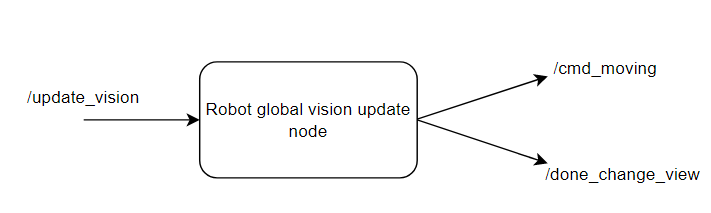
\includegraphics[width=1\textwidth]{Robot_Global_Vision_Update/RGVU_node_pub_sub.png}
		\caption{Topics are published or subscribed by Robot Global Vision Update}
	\end{figure} \\ \\ \\
	About topics which registered to publish:
	\begin{itemize}
		\item /done\_change\_view: is the topic used to publishing/subscribing requests to recognize the actual coordinates from objects on the camera view. After Robot Global Vision Update initialized, it will send to this topic the goal coordinates entered by the user with the format "[\{x coordinate\}, \{y coordinate\}]".
		\item /cmd\_moving: is the topic used to publishing/subscribing messages which is a set of points to move to. After determining the next point to go to, Robot Global Vision Update will send a message to this topic which has the format is a set of points with the first point being the current coordinates of the robot and the remaining points being the points that the robot has to go through.
	\end{itemize}
	About topics that have been registered for subscription:
	\begin{itemize}
		\item /update\_vision: is the topic used to publishing/subscribing a message containing the coordinates of a mapped destination or a confirmation message that notices the robot moved to the next point. Robot Global Vision Update subscribes to this topic to receive information about the mapped destination coordinates and passed a message to start the calculation and return the next set of points to go to.
	\end{itemize}
	
	\subsubsection{Flow chart}
	abc
	\subsubsection{State machine}
	abc
	\subsubsection{Algorithms are applied}
	Since the Autonomous Robot system applies the method of moving according to the sets of points in unknown environment, it is very important to prioritize choosing safe open points. The open points must ensure the safety of the robot during and after moving. In addition, the travel distance must be optimized to save the robot's power energy. \\
	Therefore, Robot Global Vision Update component applied algorithms to process data, involved in:
	\begin{itemize}
		\item Processing obstacles taken from SLAM map through Canny algorithm.
		\item Determining open sights and local open points at the current position of the Robot.
		\item Saving open points to visibility graph and reconstruct graph.
		\item Find next point to go to and approximately path to go to next point with has optimal distance.
		\item Remove the non-optimal points inside approximately path.
	\end{itemize}
	\paragraph{Processing obstacles taken from SLAM map through Canny algorithm\\}
	SLAM map is the image returned after the SLAM algorithm processes the data scanned by Lidar. We used Canny algorithm to analyse SLAM map and it return a list of obstacles, which are represented by a list of points that are the coordinates of the obstacle's vertices. \\
	The algorithm determines the open area based on the obstacles inside robot vision (has value between $120mm - 3,500mm$, default is $1,000mm$). However, obstacles taken from the SLAM map is not a true polygon in the geometry theory, it has noisy vertices that form redundant edges, which affects the algorithm to enlarge the obstacles (Described in detail below).
	\begin{figure}[!h]
		\centering
		
\includegraphics[width=0.7\textwidth]{Robot_Global_Vision_Update/RGVU_original_obstacle.png}
		\caption{Obstacle which has redundant edges}
	\end{figure} \\
	Regarding the concept of an obstacles represented by a set of points, we convention that all obstacles applied in the program are polygon satisfying the following two conditions:
	\begin{itemize}
		\item There is no three collinear vertices lying on the same line. Experimentally, we saw that there are four possible cases of three collinear vertices.
		\begin{figure}[!h]
			\centering
			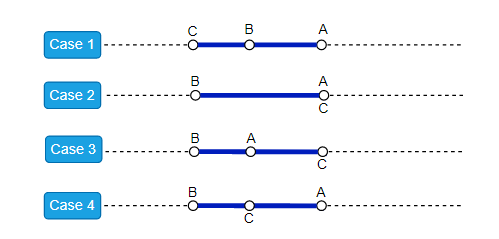
\includegraphics[width=0.7\textwidth]{Robot_Global_Vision_Update/RGVU_4case_thanghang.png}
			\caption{Four cases that 3 collinear vertices in order A$\rightarrow$B$\rightarrow$C}
		\end{figure}
		
		\item There is no two sides cross each other. Experimentally, we find that this condition is always true for the obstacles after being processed by Canny algorithm.
		\item The obstacle is a polygon with no internal holes. This condition means that in a set of points of the obstacle, the begin and the end points always coincide.\\
		\begin{figure}
			\centering
			\subfloat[\centering Obstacle is not true polygon]{{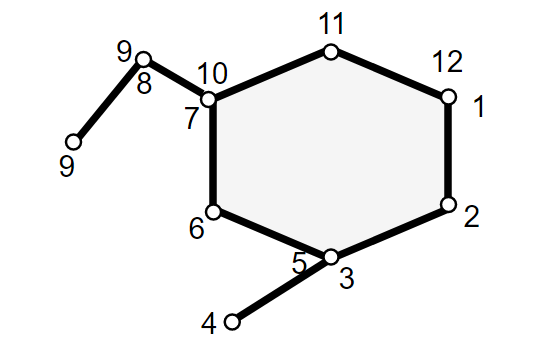
\includegraphics[width=6cm]{Robot_Global_Vision_Update/RVGU_false_ob.png} }}%
			\qquad
			\subfloat[\centering Obstacle is true polygon]{{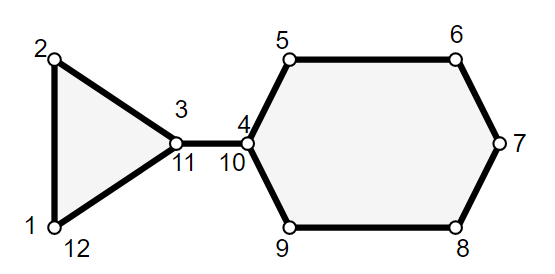
\includegraphics[width=6cm]{Robot_Global_Vision_Update/RVGU_true_ob.png} }}%
			\caption{List of obstacle with vertex numbers as the index in list}
			\label{fig:my_label}
		\end{figure}
	\end{itemize}
	
	Based on the conventions about obstacles that described above, we implemented a data preprocessing strategy before applying the obstacle zoom in algorithm. The data preprocessing algorithm we implemented is described by the following pseudo code: \\
	\begin{algorithm}
		\caption{Obstacles preprocessing}
		\begin{algorithmic}[1]
			\REQUIRE obstacles list
			\ENSURE obstacles list which NOT EXIST 3 vertex in a line for each obstacle
			\Statex
			\Function{preprocess\_obstacles}{$obstacles$}:
			\FOR{each \texttt{obstacle} in \texttt{obstacles}}
			\FOR{$index \gets 0\ to\ lenght(obstacle) - 2$}
			\STATE $previous\_vertex \gets obstacle[index - 1]$
			\STATE $current\_vertex \gets obstacle[index]$
			\STATE $after\_vertex \gets obstacle[index + 1]$
			\STATE $AB \gets point\_distance(previous\_vertex, current\_vertex)$
			\STATE $AC \gets point\_distance(current\_vertex, after\_vertex)$
			\STATE $BC \gets point\_distance(previous\_vertex, after\_vertex)$
			\IF{$AB + AC == BC$}
			\STATE $obstacle.pop(index)$
			\ELSIF{$AC + BC == AB$}
			\STATE $new\_vertex \gets current\_vertex + normal_vector(current\_vertex, after\_vertex)$
			\STATE $obstacle.append(index + 1, new\_vertex)$
			\STATE $obstacle.append(index + 2, previous\_vertex)$
			\STATE $index \gets index + 2$
			\ELSIF{$AB + BC = AC$}
			\STATE $new\_vertex \gets current\_vertex + normal_vector(current\_vertex, after\_vertex)$
			\STATE $obstacle.append(index + 1, new\_vertex)$
			\STATE $index \gets index + 1$
			\ENDIF
			\ENDFOR
			\ENDFOR
			\EndFunction
		\end{algorithmic}
	\end{algorithm}
	
\end{document}